% ==============================================================================
\documentclass[12pt]{gsis} % 12pt font required by GSIS;
\usepackage[misc]{ifsym} 
\usepackage{graphicx,subfigure}
\usepackage{hyperref,caption}
\usepackage[para,online,flushleft]{threeparttable}
\usepackage{multirow,booktabs}
\usepackage{indentfirst}
\usepackage{geometry}
\usepackage{natbib}
\captionsetup[figure]{justification=centering}
\bibpunct[, ]{(}{)}{;}{a}{}{,} % Citation support using natbib.sty

% ==============================================================================
\begin{document}

\copyrightyear{2023}
\datereceived{ Nov 28th 2023}
\dateaccepted{ Nov 28th 2023}

%%% Full title of the paper (Capitalized)
\title{Metro Impact on the Property Value of Surrounding Areas: A Case Study in São Paulo, Brazil}

%%% Authors and Affiliations 
\author[a]{Guilherme F. Alves}
\affil[a]{Department of Transport Engineering at the Polytechnical School, University of São Paulo, São Paulo, Brazil.}

%%% Contact information of the corresponding author
\thanks{\textbf{CONTACT:} Guilherme Fernandes Alves  \quad \Letter : gf10.alves@gmail.com}

%%% Keywords
\keywords{Urban Metro Impact; Real Estate Valuation; Spatial Econometrics}

%%% Abstract 
\Abstract{This study investigates the influence of metro networks on property values in São Paulo, Brazil, leveraging extensive data on property tax (IPTU) and real estate valuation from 1995 to the present. The research adopts spatial econometric methods, combining data science and spatial analysis, to explore the relationship between metro accessibility and residential property prices. The results indicate a non-linear, positive correlation between metro proximity and property valuation, aligning with global urban development trends. This paper contributes valuable insights into urban metro impacts on real estate, offering implications for urban planning and policy-making in rapidly urbanizing cities.}

%%% GSIS inner commands
\newgeometry{top=20.0mm,bottom=40.0mm,left=15mm,right=15mm,headsep=8mm}
\maketitle
\restoregeometry
\newpage
% ==============================================================================

\section{Introduction}
This document describes a research project from the `Geospatial Data Science' course at the University of São Paulo, under supervision of the Professor Mariana Giannotti.
The course teaches students to combine data science with spatial analysis.
After foundational data science instruction and practical labs, students apply their knowledge to a project of their choice.
This project examines how metro networks affect nearby property values.

The Brazilian `\textit{Imposto Predial e Territorial Urbano}' (IPTU), also known as the `Property Tax', is a tax collected every year from property owners in Brazil.
This tax data, along with property values, is released annually by the Government of each city, including the city of São Paulo.
Records are available from 1995 to the present.
This extensive dataset enables studies on how the metro network influences property values in nearby areas.

The paper starts with a literature review, which was not exactly the purpose of the course so it may be a bit shorter than expected.
Next, the methods used to conduct the analysis are described in detail, allowing for the replication of the study if desired.
Results are then shared and discussed, and the paper ends with the concluding remarks.
Notably, there is an appendix section to save valuable information that may not be necessary for understanding the research.
% This was created mainly to avoid the reader to be distracted by too much information in the main text.

\section{Literature Review}

The impact of metro accessibility on residential property values is a topic of growing importance in urban planning and economic studies.
Given this context, the work of \citet{LI201852} provides valuable insights for the city of Xi'an, China.
The study's main finding is a generally positive, non-linear relationship between proximity to metro stations and property values.
The greatest increase in property values is observed at distances ranging from 300 to 1,200 meters from metro stations.
% In contrast, areas immediately adjacent to the stations see a lesser increase, likely due to negative factors such as noise and congestion.

In a similar fashion, the research conducted by \citet{sun2016impact} investigates the influence of subway line construction on residential property values in Tianjin, China.
Utilizing an Hedonic Pricing Model, this study examines the changes in property values within a 1km radius of the newly completed subway line 3 stations.
The findings revel a positive impact of subway lines on surrounding property values, with a more noticeable effect in the outskirts than in downtown areas.
This suggests that the impact of subway construction on residential prices varies across different areas of the city.

Contrasting with the aforementioned studies, the research by \citet{campos_almeida_2018} focuses on São Paulo, Brazil.
This study aims to decompose the implicit effects, neighborhood, and adjacency in influencing property prices both within and between properties, as well as districts.
The results reveal that a significant portion (96.89\%) of the property price is determined by intrinsic and locational characteristics, while a smaller fraction (3.11\%) is attributed to neighborhood and adjacency effects, including the characteristics of the districts and spatial spillover among them.
% This highlights the predominant influence of the property's own characteristics and its location over the district's characteristics.

Based on these insights, this study seeks to quantify the impact of metro stations on surrounding property values in São Paulo.
An equation will be proposed to estimate property values, incorporating the distance to the metro network and its temporal dynamics.

\section{Methods}

% \subsection{Data}

It is worth to start this section by mentioning the dataset used.
The IPTU data from São Paulo is publicly available.
However, a significant effort have been made by \citet{Gomes_2022} to condense this data, enhancing its usability.
Specifically, this study utilizes the summarized property values per transport zone for each year, without any alterations.

% \subsection{Clustering}

To start conducting the analysis, the official transport zones of the city of São Paulo, provided by the São Paulo Metro Company \citep{MetroSP2017Pesquisa}, were used.
This segmentation of the city is created aiming the analysis of origin-destination matrices of the public transport network, which are build every 10 years for the city of São Paulo.
For this study, the data from 2017 was used, which is the most recent one.
Along with the spatial data, different variables are also included in the dataset, such as the number of inhabitants, number of jobs, and number of households.

Socio-economic variables relevant were chosen for clustering the transport zones.
These variables include population, school enrollments, employment, area (in hectares), and per capita income.
To run the clustering operation, the k-means method \citep{macqueen1967some} was selected due to its simplicity and ease of interpretation.

Determining the optimal number of clusters is not a trivial task, and there are many methods to do so.
Although different optimization schemas were considered [e.g. the kneed algorithm \citep{Arvai_kneed_2020}], the final number of clusters was selected based on the ease of interpretation of the results.
In this case, the number of clusters was constrained up to 5, which is a reasonable number of groups to be analyzed and interpreted.
Sensitivity analysis was conducted to understand the best number of clusters within the range of 2 to 5.

% \subsection{Spatial Autocorrelation}

The next step involves validating the hypothesis that property values are influenced by geographic location.
This was examined using the Moran's I test \citep{moran} for spatial autocorrelation of property values.

% \subsection{Variables Construction}

After validating the autocorrelation of property values within the city, it was necessary to construct the variables for the final model.
The first important variable is the distance to the metro network.
To accomplish this, a dataset representing all the metro stations built up to each year in the analysis was constructed.
Determining the inauguration date of each metro station was crucial, made possible by the dataset provided by \citet{kaggle_dataset}.

The transport zones remain unchanged over the years.
For each zone, its centroid was first calculated.
Then, varying the years, the distance from the centroid of each zone to the 10th closest metro station was calculated for each year.
This approach was applied to each transport zone and for each year.
Considering the 10th closest metro station was important to ensure significant variability in the constructed variable, thereby improving the model's quality.

% \begin{equation}\label{eq:distance}
%     \text{Dist}_{i,10,y} = D\left(C_i, M_{10,y}\right)
% \end{equation}

Additionally, it was necessary to convert the property values, available for each year, to their present value.
This was done using the national inflation index, IPCA, obtained from the Brazilian Institute of Geography and Statistics (IBGE), the official index provider.

First, the IPCA for each month, ranging from 1981 to the present, was provided.
However, it was necessary to convert this to an annual IPCA.
This conversion was achieved by calculating the equivalent annual interest rate, as expressed by equation (\ref{eq:ipca}).
%
\begin{equation}\label{eq:ipca}
	IPCA_{year} = \prod_{i=1}^{12} (1 + IPCA_{month_i}) - 1
\end{equation}

where $IPCA_{year}$ is the annual IPCA, and $IPCA_{month_i}$ is the IPCA for the $i$th month of the year.

The property values were converted by applying the annual interest rate for each year up to the present, as expressed by equation (\ref{eq:property_value}).
%
\begin{equation}\label{eq:property_value}
	PropertyValue_{present} = PropertyValue_{year} \times (1 + IPCA_{year})^{(year_{present} - year)}
\end{equation}

% \subsection{Visualization}

Visualizing the data is crucial for understanding the distribution of variables and identifying possible outliers.
This step is challenging, as the outcome variables may be excessively noisy, affecting the visualization.
To address this issue, a Savitzky-Golay filter \citep{savitzky1964smoothing} to smooth the data and make it easier to visualize without losing the main characteristics of the data.

% \subsection{Model}

Finally, to build the model, an exponential regression model was required, as expressed by equation (\ref{eq:exponential}).
%
\begin{equation}\label{eq:exponential}
	z = \beta_0 \times e^{\beta_1 \times x + \beta_2 \times y}
\end{equation}

where $z$ is the property value, $x$ is the distance to the metro network, and $y$ is the time.

Before moving to the next section, it important to notice that all the code used to conduct this analysis is available on \href{https://github.com/Gui-FernandesBR/MetroImpactOnPropertyValues}{GitHub}, thus allowing for future replication or enhancements of the study.

\section{Results and discussion}

The parameters and coefficients obtained from the model are as follow.
The first coefficient for distance to the metro network is -0.00018.
The second coefficient, related to time, is 0.020941040.
Intercept: The model's intercept is found to be -34.390.

These finding reveal that 0.00018 is the rate of change of the property value as the distance to the metro network increases.
In other words, the property value decreases by 0.00018 for each meter away from the metro network.
Similarly, the property value increases by 0.020941040 for each year that passes by.

Figure \ref{fig:property-value} allows one to visualize these results, showing the actual property values (post-filtering) as blue dots and the exponential fit as a surface, with values associated with a color scale.

\begin{figure}[ht]
	\centering
	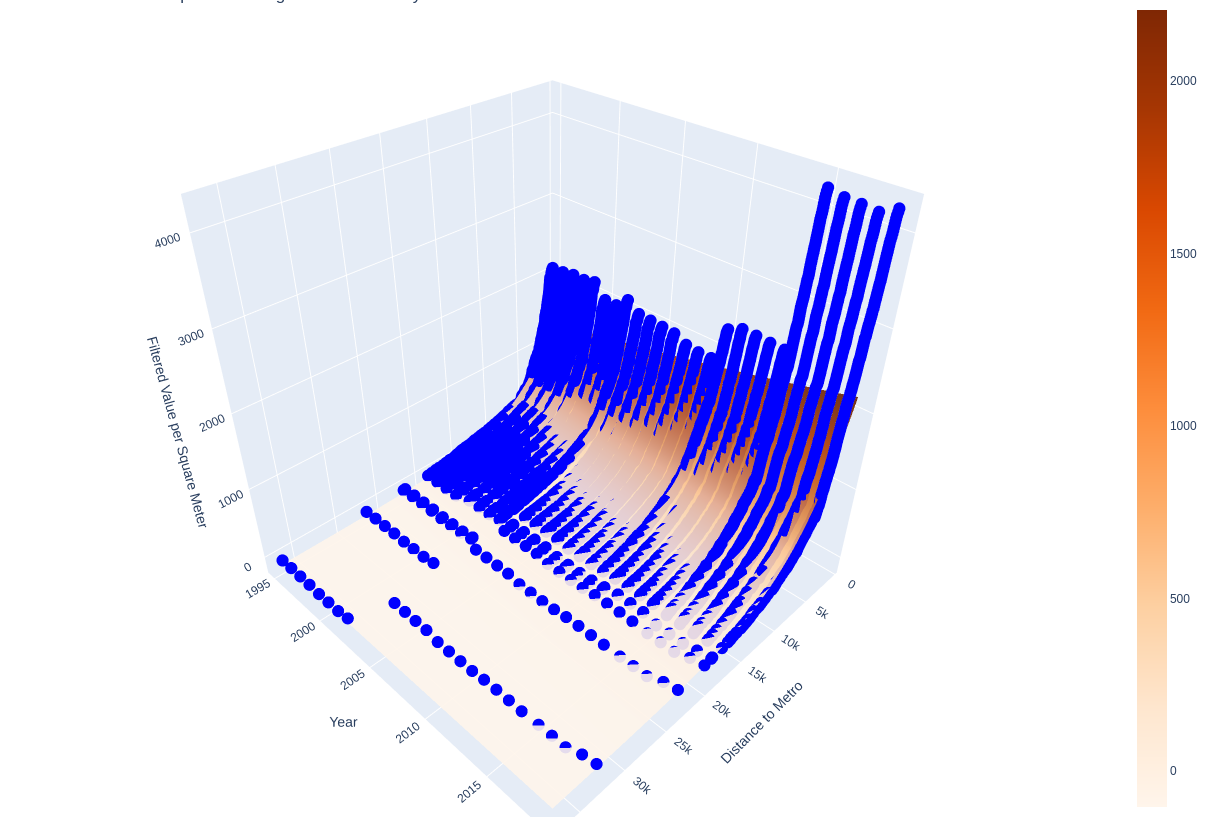
\includegraphics[width=0.8\textwidth]{figs/exponential_regression.png}
	\caption{- Property value as a function of the distance to the metro network and the time. The blue dots are the actual values after filtering, and the surface is the exponential fit with its values associated to the color scale.}
	\label{fig:property-value}
\end{figure}

Overall, as expected, the property values increases as the distance to the metro network decreases.
Also, the property value increases as the time passes by, which is a good indicator of the inflation of the property value.
% Overall the results are in line with the literature, and the model is able to explain significant part of the property value.

The goodness of fit of the model was found as $78.12\%$ when comparing the predicted values against the real values.

It is noticeable that the exponential fit is a good option to model the property value based on the distance to the metro network and the time.
Nevertheless, It is important to note that the metro network is not the only variable that may impact the property value.
This constitutes a limitation of the model, as variables intrinsic to the property itself, such as the number of rooms, may also impact the property value but were not considered in this study since they were not available in the dataset.

As a cavear, it is valuable commenting that the influence of the metro network on the property value decreases as the distance to the metro network increases, achieving a point where this influence is negligible.
This could be used to estimate the maximum distance to the metro network where the property value is still impacted by the metro network, thus providing a valuable information for the city planners and future researches.

\section{Concluding remarks}

By the end of this study, it was possible to conclude that the metro network has a positive impact on the property value of the surrounding areas.
This is in line with the literature, and the model was able to explain significant part of the property value.

To future research on top of this study, it is suggested to consider other variables that may impact the property value.
Alternatively, investigating the change of land cover over time and its relationship with the metro network may also be an interesting research topic.
LiDAR data could be used to extract the land cover information, and the metro network could be used as a proxy for the urbanization of the city.
As a last suggestion, a predictor function could be built to estimate the property value for residences near to the planned future metro stations.

Finally, it is worth to mention that this article has been written for a specific course at the University of São Paulo, and the author is open to suggestions and corrections.
Sending the content to an international journal or conference was not the initial intention, but it is not discarded.
If that is the case, a second author may be needed.

% ==============================================================================

%%% References 
\bibliographystyle{abbrvnat} % Or any other style you prefer, like apalike, abbrvnat, etc.
\bibliography{ref}

\section{Appendix}

Consider this section as a place to save valuable information that may not be included in the main text.
Reading this section is not mandatory for completely understanding the research.

Finally, we emphasize that the work has been made available on-line and any contributions are welcome.
The smallest, but still valuable, contribution is to star the repository on \href{https://github.com/Gui-FernandesBR/MetroImpactOnPropertyValues}{GitHub}.

\begin{figure}[ht]
	\centering
	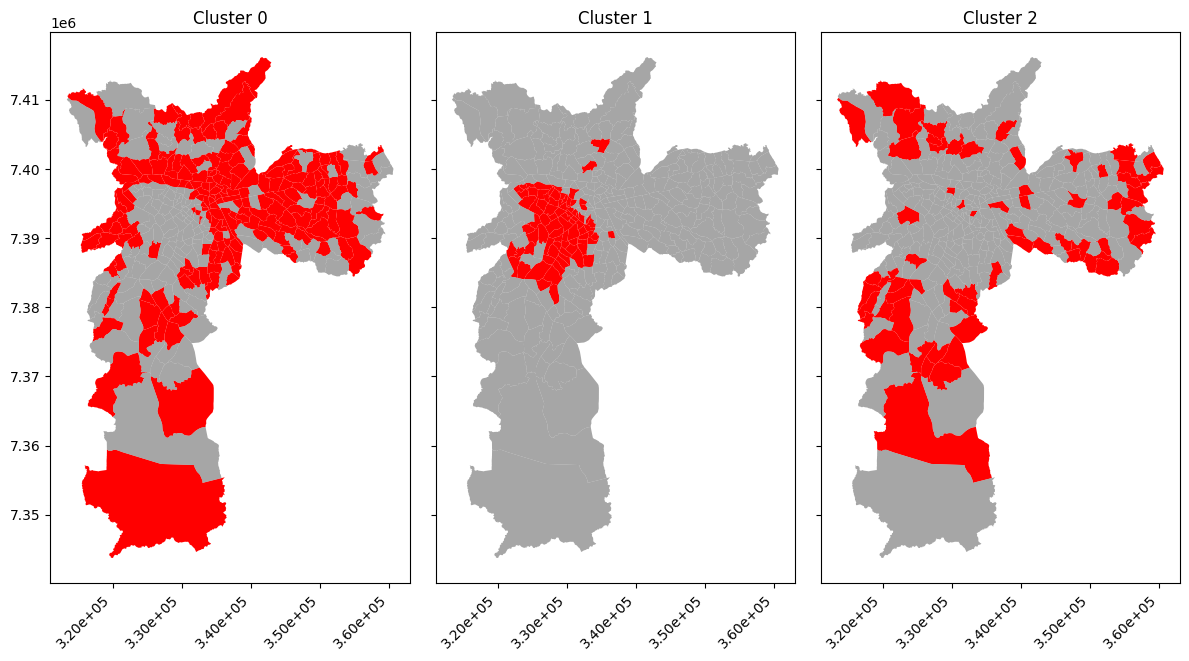
\includegraphics[width=0.8\textwidth]{figs/cluster-3.png}
	\caption{- Cluster analysis of the transport zones of the city of São Paulo based on socio-economic variables. The number of clusters was selected based on the ease of interpretation of the results.}
	\label{fig:cluster}
\end{figure}

\begin{figure}[ht]
	\centering
	\subfigure[Actual Data]{
		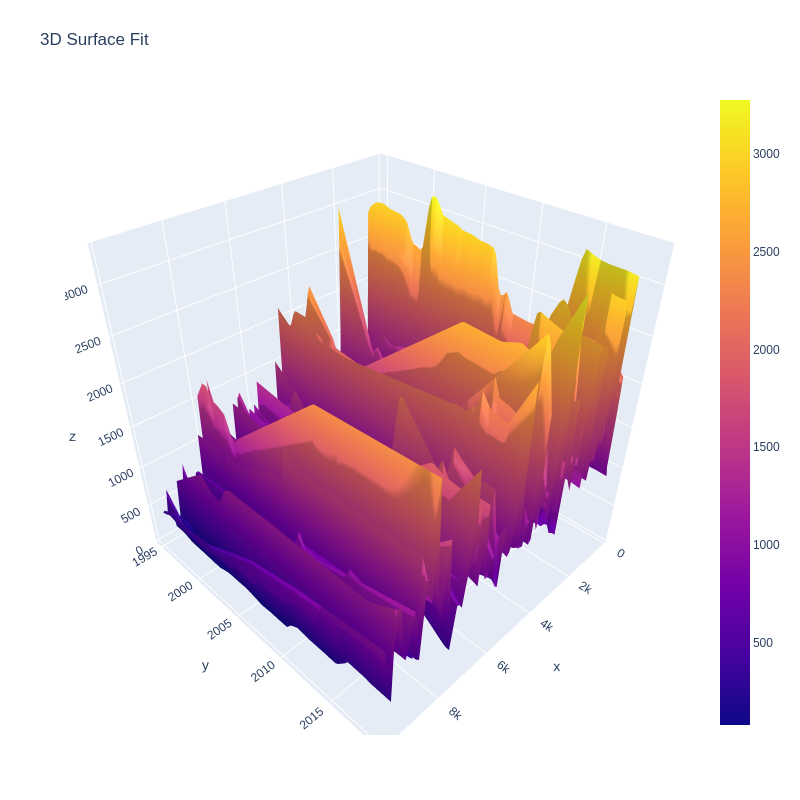
\includegraphics[width=0.45\textwidth]{figs/non_filtered.png}
		\label{fig:property-value-normal}
	}
	\subfigure[Filtered Data]{
		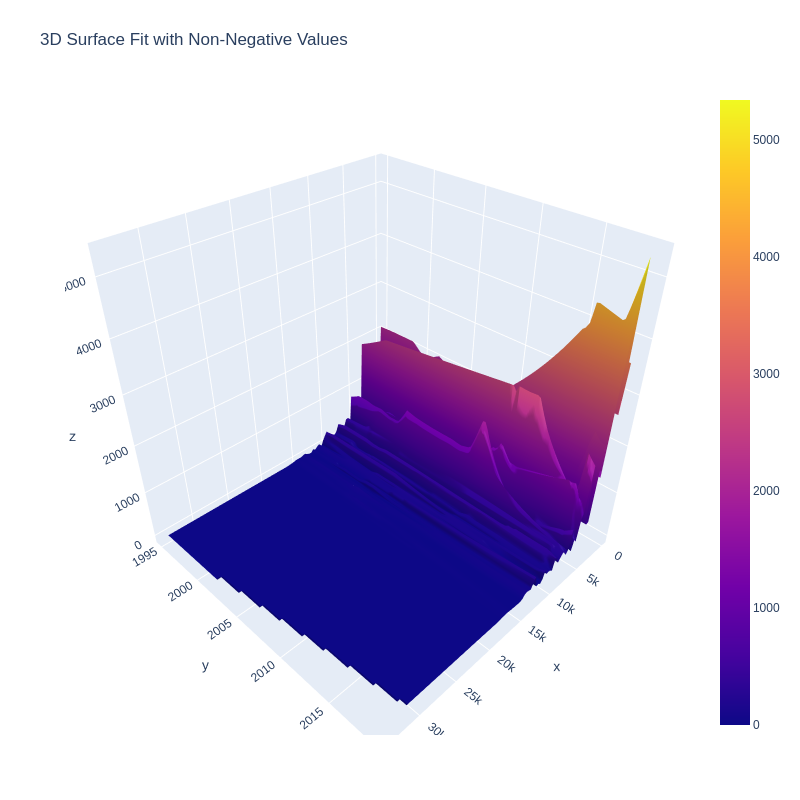
\includegraphics[width=0.45\textwidth]{figs/filtered.png}
		\label{fig:property-value-filtered}
	}
	\caption{- Property value as a function of the distance to the metro network and the time.}
	\label{fig:comparison}
\end{figure}

\begin{figure}[ht]
	\centering
	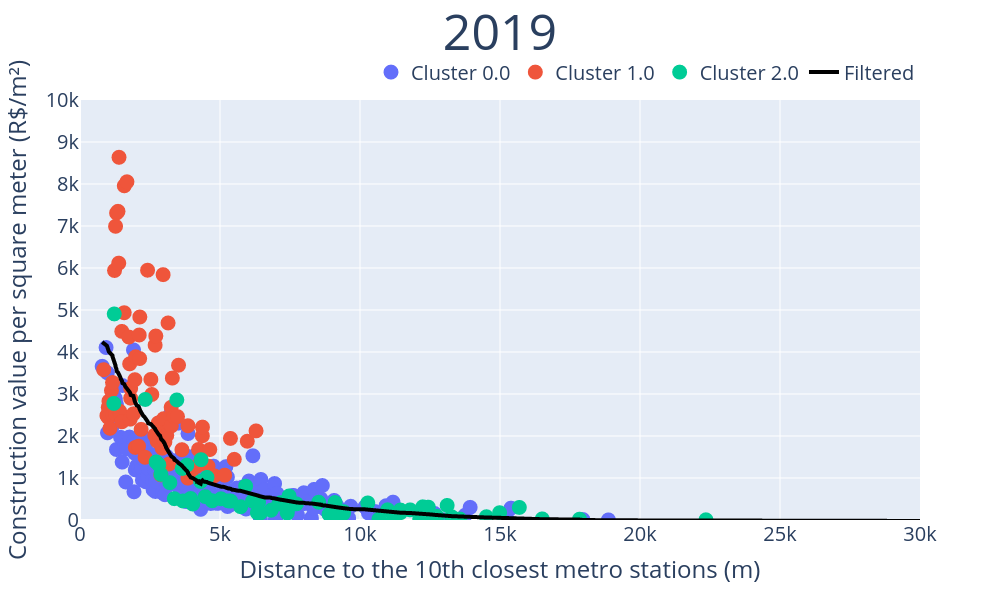
\includegraphics[width=0.8\textwidth]{figs/clusters_2019.png}
	\caption{- 2D plot of the constructed area for each transport zone in the city of São Paulo. The color of the points represents the cluster to which the transport zone belongs. Cluster 1 is the central area of the city, typically with higher property values.}
\end{figure}

\end{document}